% Autor: Leonhard Segger, Alexander Neuwirth
% Datum: 2017-10-30
\documentclass[
	% Papierformat
	a4paper,
	% Schriftgröße (beliebige Größen mit „fontsize=Xpt“)
	12pt,
	% Schreibt die Papiergröße korrekt ins Ausgabedokument
	pagesize,
	% Sprache für z.B. Babel
	ngerman
]{scrartcl}

% Achtung: Die Reihenfolge der Pakete kann (leider) wichtig sein!
% Insbesondere sollten (so wie hier) babel, fontenc und inputenc (in dieser
% Reihenfolge) als Erstes und hyperref und cleveref (Reihenfolge auch hier
% beachten) als Letztes geladen werden!

\usepackage{tikz}
\usetikzlibrary{calc,patterns,angles,quotes} % loads some tikz extensions\usepackage{tikz}
\usetikzlibrary{babel}

% Silbentrennung etc.; Sprache wird durch Option bei \documentclass festgelegt
\usepackage{babel}
% Verwendung der Zeichentabelle T1 (Sonderzeichen etc.)
\usepackage[T1]{fontenc}
% Legt die Zeichenkodierung der Eingabedatei fest, z.B. UTF-8
\usepackage[utf8]{inputenc}
% Schriftart
\usepackage{lmodern}
% Zusätzliche Sonderzeichen
\usepackage{textcomp}

% Mathepaket (intlimits: Grenzen über/unter Integralzeichen)
\usepackage[intlimits]{amsmath}
% Ermöglicht die Nutzung von \SI{Zahl}{Einheit} u.a.
\usepackage{siunitx}
% Zum flexiblen Einbinden von Grafiken (\includegraphics)
\usepackage{graphicx}
% Abbildungen im Fließtext
\usepackage{wrapfig}
% Abbildungen nebeneinander (subfigure, subtable)
\usepackage{subcaption}
% Funktionen für Anführungszeichen
\usepackage{csquotes}
\MakeOuterQuote{"}
% Zitieren, Bibliografie
\usepackage[sorting=none]{biblatex}


% Zur Darstellung von Webadressen
\usepackage{url}
%chemische Formeln
\usepackage[version=4]{mhchem}
% siunitx: Deutsche Ausgabe, Messfehler getrennt mit ± ausgeben
\usepackage{floatrow}
\floatsetup[table]{capposition=top}
\usepackage{float}
% Verlinkt Textstellen im PDF-Dokument
\usepackage[unicode]{hyperref}
% "Schlaue" Referenzen (nach hyperref laden!)
\usepackage{cleveref}
\sisetup{
	locale=DE,
	separate-uncertainty
}
%\bibliography{BA-C-04_V05_08-04-2019_References}
%TODO aktivieren

\begin{document}

	\begin{titlepage}
		\centering
		{\scshape\LARGE Versuchsbericht zu \par}
		\vspace{1cm}
		{\scshape\huge V05 - Titel \par} %TODO Anpasen
		\vspace{2.5cm}
		{\LARGE Gruppe BA-C-04 \par}
		\vspace{0.5cm}

		{\large Alexander Neuwirth (E-Mail: a\_neuw01@wwu.de) \par}
		{\large Leonhard Segger (E-Mail: l\_segg03@uni-muenster.de) \par}
		\vfill

		durchgeführt am 08.04.2019\par
		betreut von\par
		{\large Raffaela Busse} \par
		und \par
		{\large Daniel Guderian}
		\vfill

		{\large \today\par}
	\end{titlepage}
	\tableofcontents
	\newpage

	%TODO mehr TODO in Default

	\section{Kurzfassung}
	% Hypothese	und deren Ergebnis, wenn Hypothese ist, dass nur Theorie erfüllt, sagen: Erwartung: Theorie aus einführung (mit reflink) erfüllt
	% Ergebnisse, auch Zahlen, mindestens wenn's halbwegs Sinn ergibt
	% Was wurde gemacht
	% manche leute wollen Passiv oder "man", manche nicht

  \section{Theorie}
	% wdh. Texte
	% wdh. Besprechung

	\section{Methoden}
	% Bilder von der Website klauen
	% einer will Präsens

	%TODO  Zeiten
	% Zeitdifferenz: 25.3h
	% Positronium_Zeitdifferenz: 1.2h
	% Zeitkalibrierung: 7s
	% Energy_Start: 3.7m
	% Energy_Stop: 11.4m

	%TODO
	% Zeit in Material bei Speed of Light vernachläsigbar (bzw. Ausdehnung)

	\section{Ergebnisse und Diskussion}
	%TODO Unsicherheiten


	\subsection{Beobachtung und Datenanalyse}
	% Allgemeine Beobachtungen
	% Einflüsse von veränderten Parametern auf Messung
	\subsubsection{Unsicherheiten}
	% Berechung nach Aufgabenstellung

	\subsection{Energiespektren}
	Zuächst wurden die Energeispektren \cref{fig_energy_start} und \cref{fig_energy_stop} gemessen. Hieraus wurden die Kanalbereiche für aus dem jeweiligen Prozess stammende Photonen ermittelt.

	%TODO Peaks der zwei Zerfälle nicht unterscheidbar

	\begin{figure}[H]
				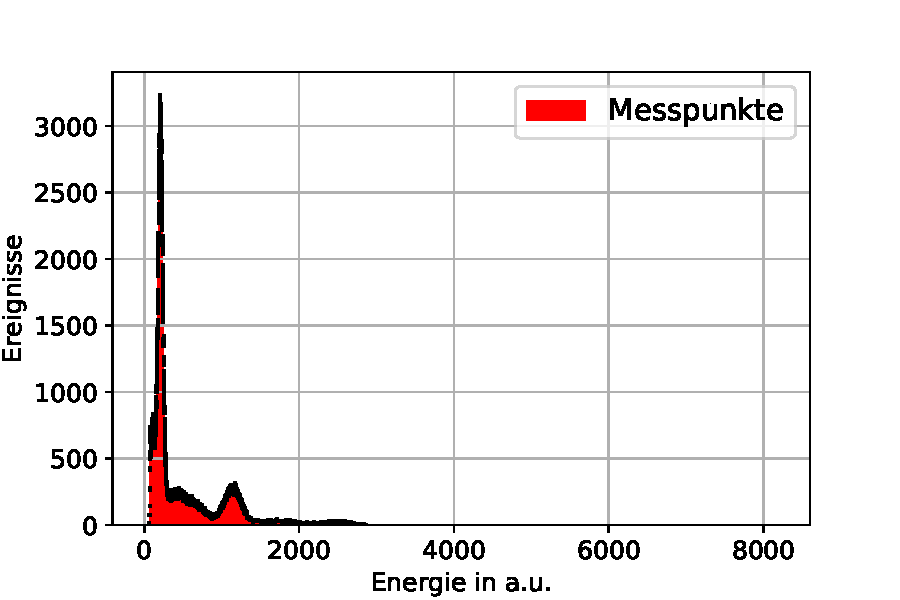
\includegraphics[width= 0.9 \linewidth]{img/Energiespektrum_Start}
				\caption{
				Energiespektrum welches von der ersten Messapparatur aufgenommen wurde.
				Die Unsicherheiten sind in Schwarz abgebildet, sodass sich der Messwert mittig im schwarzen Bereich befindet.
				}
				\label{fig_energy_start}
		\end{figure}

	\begin{figure}[H]
				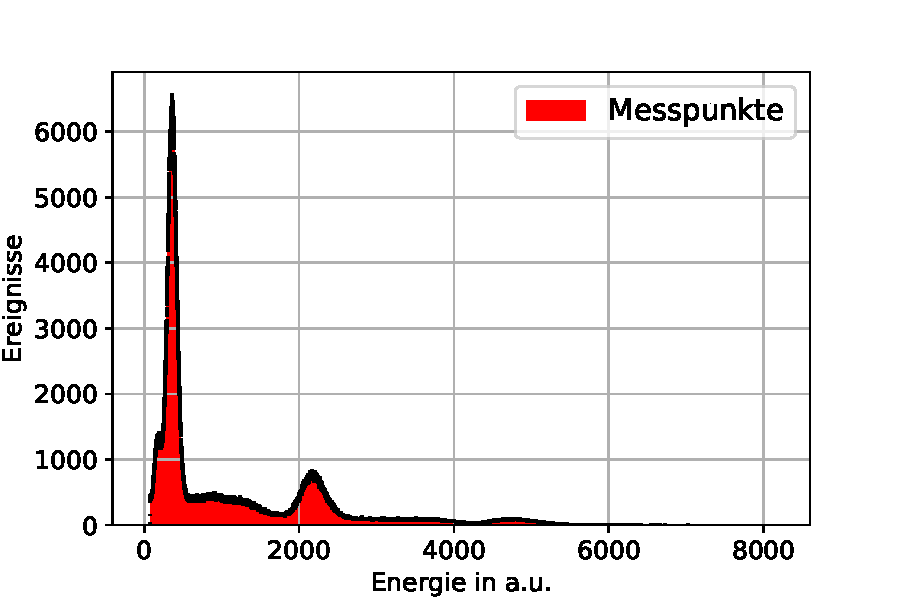
\includegraphics[width= 0.9 \linewidth]{img/Energiespektrum_Stop}
				\caption{
				Energiespektrum welches von der zweiten Messapparatur aufgenommen wurde.
				Die Unsicherheiten sind in Schwarz abgebildet, sodass sich der Messwert mittig im schwarzen Bereich befindet.
				}
				\label{fig_energy_stop}
		\end{figure}

  \subsubsection{Zeitkalibrierung}
	Der Mittelwert der Abstände der Peaks in \cref{fig_zeitkalibrierung} beträgt \SI{514.8+-0.4}{}, das heißt so viele Kanäle entsprechen einer Zeit von \SI{0.64+-0.003}{\mu s}.

	\begin{figure}[H]
				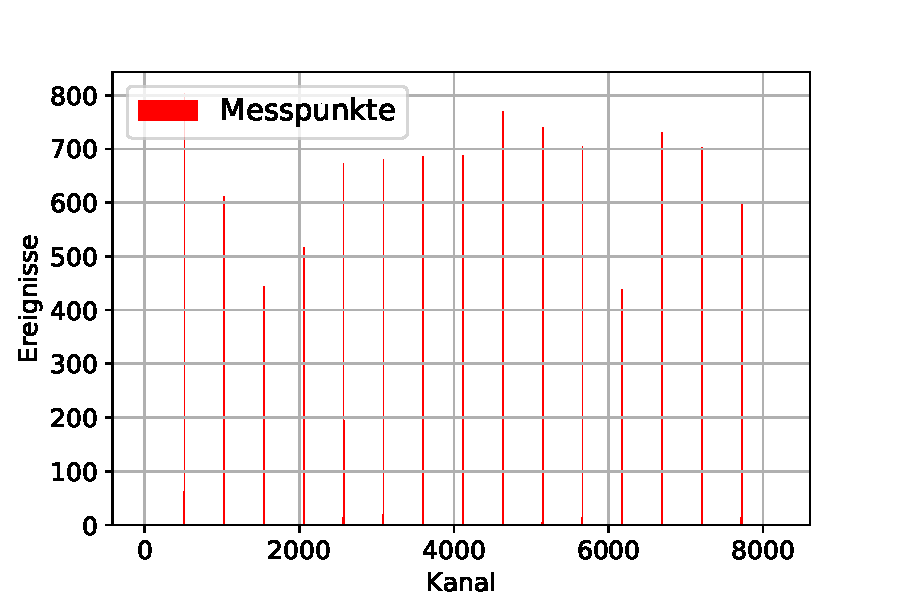
\includegraphics[width= 0.9 \linewidth]{img/Zeitkalibrierung}
				\caption{
				Zeitkalibrierung der Kanäle mittels eines Zeitkalibrators %TODO 'TIME Calibrator' ?
				Es gibt auch kleine Beiträge zu anderen Kanälen in naher Umgebung der Peaks, jedoch sind diese wegen der Auflösung des Bildes kaum sichtbar.
				}
				\label{fig_zeitkalibrierung}
		\end{figure}

		\subsubsection{Bestimmung des Nullpunkts}
		In \cref{fig_positronium_zeitdifferenzen} sind die Messungen der Zeitdifferenzen des Positroniumzerfalls abgebildet.
		Da dieser sehr scharf ist, ist er in \cref{fig_positronium_zeitdifferenzen_zoom} vergrößert dargestellt.
		Es wird eine Gaußfunktion \ref{eq_gauss} an die Messpunkte angepasst.
		\begin{equation}
			\label{eq_gauss}
			%A * np.exp(-(x - x0)**2 / 2 / d**2)
			 f(t) = N\exp\left\{{\frac{(t-T_0)^2}{2 \Delta T^2}}\right\}
		\end{equation}
		Die Standardabweichung des Fits $\Delta T$ beschreibt für die folgende Bestimmung der Lebensdauer des $\gamma$-Niveaus die Unsicherheit der Messapparatur bei der Auflösung von Zeitdifferenzen, da beim Positroniumzerfall kein zeitlicher Unterschied vorliegt. %TODO ref in Theorie? bzw. vernachlässigbar klein

	\begin{figure}[H]
				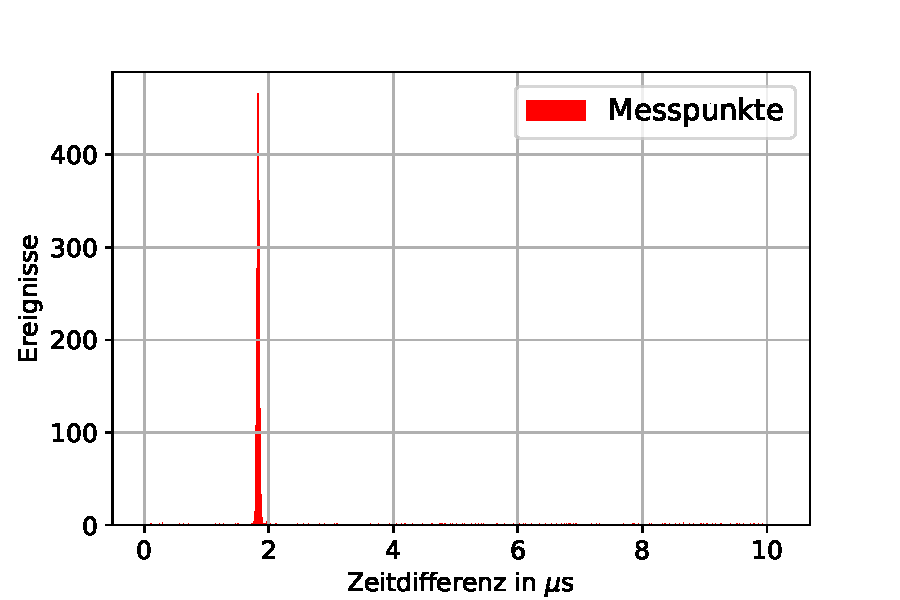
\includegraphics[width= 0.9 \linewidth]{img/Positronium_Zeitdifferenz}
				\caption{
					Positronium-Kanal
				Die Unsicherheiten sind in Schwarz abgebildet, sodass sich der Messwert mittig im schwarzen Bereich befindet.
				}
				\label{fig_positronium_zeitdifferenzen}
		\end{figure}

	\begin{figure}[H]
				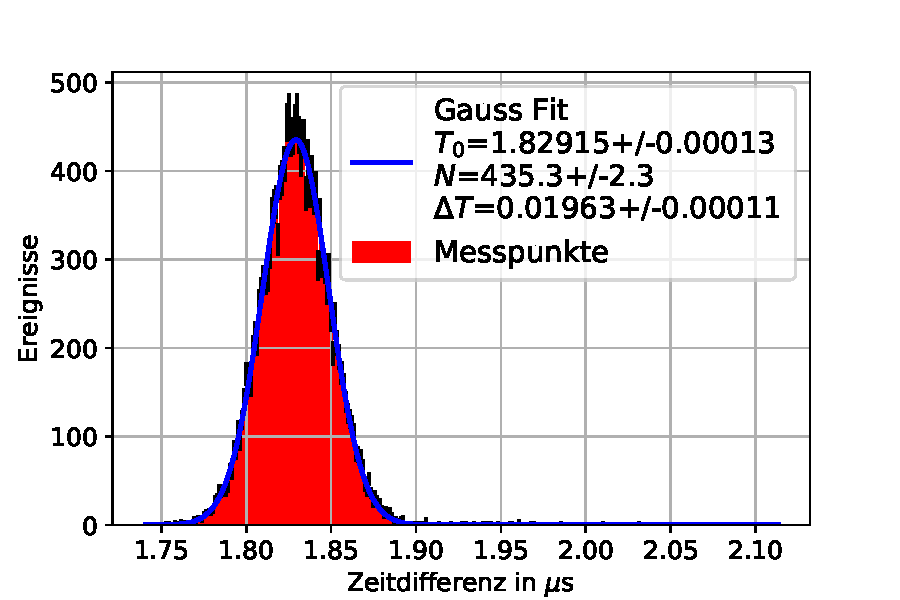
\includegraphics[width= 0.9 \linewidth]{img/Positronium_Zeitdifferenz_zoom}
				\caption{
					Positronium-Kanal:
				Die Unsicherheiten sind in Schwarz abgebildet, sodass sich der Messwert mittig im schwarzen Bereich befindet.
				}
				\label{fig_positronium_zeitdifferenzen_zoom}
		\end{figure}

		\subsubsection{Bestimmung der Lebensdauer}

		\subsubsection*{Abschätzung}
		Mit \cref{fig_zeitdifferenz_zoom} wurde die Halbwertszeit grob abgeschätzt.
		Hierbei beschreibt die grüne Horizontale bei \SI{125}{} Ereignissen den Untergrund (siehe \cref{fig_zeitdifferenz}).
		In gelb verlaufen eine Horizontale und eine Vertikale durch das abgeschätze Maximum.
		Ebenso ist der Punkt der mit halb so vielen Ereignissen (ohne den Untergrund) lila markiert.
		Die Differenz gibt die Halbwertszeit $t_{1/2}=\SI{150+-50}{ns}$.
		\begin{figure}[H]
				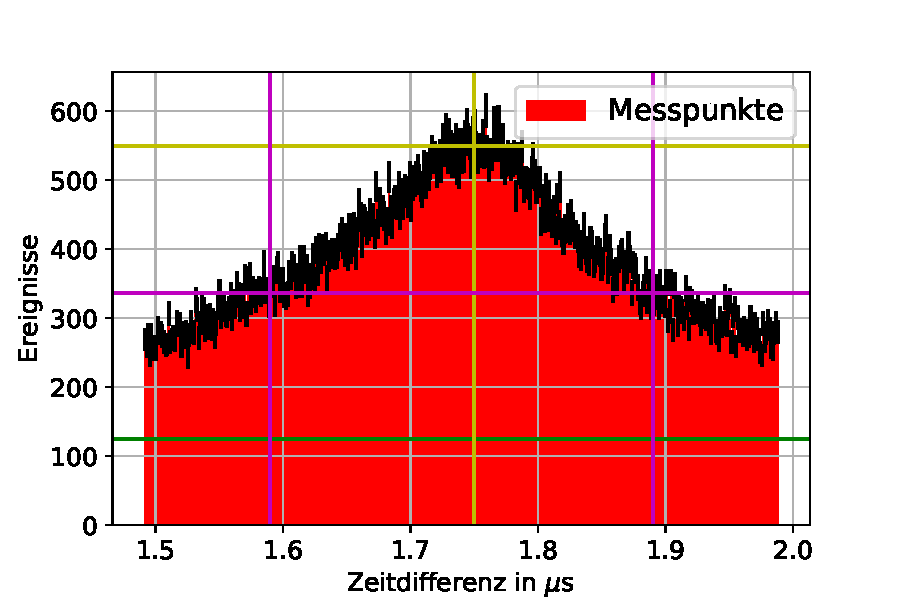
\includegraphics[width= 0.9 \linewidth]{img/Zeitdifferenzen_zoom}
				\caption{
					$\gamma$-Niveau-Kanal:
				Die Unsicherheiten sind in Schwarz abgebildet, sodass sich der Messwert mittig im schwarzen Bereich befindet.
				}
				\label{fig_zeitdifferenz_zoom}
		\end{figure}
		\subsubsection*{Fit}
		In \cref{fig_zeitdifferenz} ist die Grüne Linie der Mittelwert aller Ereignisse bei einer Zeitdifferenz größer \SI{4}{\mu s}.
		Der lila Fit ist in in die jeweilige Richtung ein exponentiell abfallende Funktion:
		\begin{equation}
			\label{eq_dexp}
			f(t)=N\cdot (\exp{-\left\{\lambda_1(t-T_0)\right\}}\Theta(t-T_0)+\exp{\left\{\lambda_2(t-T_0)\right\}}\Theta(T_0-t))
		\end{equation}
	\begin{figure}[H]
				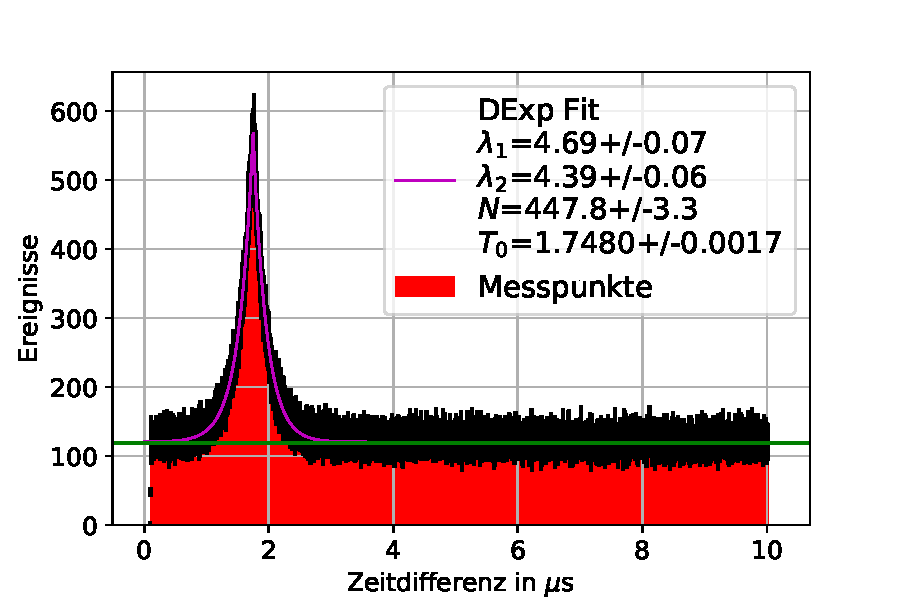
\includegraphics[width= 0.9 \linewidth]{img/Zeitdifferenzen}
				\caption{
					$\gamma$-Niveau-Kanal:
				Die Unsicherheiten sind in Schwarz abgebildet, sodass sich der Messwert mittig im schwarzen Bereich befindet.
				}
				\label{fig_zeitdifferenz}
		\end{figure}
		\subsubsection*{Mittelwert}
		Außerdem lässt sich die mittlere Lebensdauer durch
		\begin{equation}
			\label{eq_mittel}
			\tau = \frac{\sum_i t_i \cdot n_i}{\sum_i n_i}
		\end{equation}
		bestimmen.
		Wobei hier $t_i$ der Abstand zum Maximum (hier $\SI{1.74}{\mu s}$) und $n_i$ die Anzahl der Ereignisse \textbf{ohne} den Untergrund ist.
		\cref{eq_mittel} ist also der gewichtete und normierte Mittelwert der Lebesndauern und die Unsicherheit ergibtsich aus dem Quotienten der Standardabweichung und der Wurzel der Abnzahl der Messpunkte über welche gemittelt wird ($\frac{s}{\sqrt{N}}$).

		Es ergibt sich $\tau_3=\SI{230+-3}{ns}$ im Bereich von $\SI{1.74}{\mu s}$ bis $\SI{3}{\mu s}$ und umgekehrt in $\SI{0.4}{\mu s}$ bis $\SI{1.74}{\mu s}$ folgt $\tau_4=\SI{230+-4}{\mu s}$.
		Die Bereiche wurden so gewählt, da in \cref{eq_mittel} die Terme hoher $t_i$, die um Null schwanken, zu großen Fehlern führen.

		In \cref{tb_leb} sind die insgesamt resultierenden Lebensdauern aufgeführt.
		\begin{table}[H]
		\centering
		\begin{tabular}{c| c | c | c | c  }
			 Index&Methode&$\lambda$ in \si{\mu s^{-1}}& $\tau=1/\lambda$ in \si{ns} &$t_{1/2}=\tau\ln 2$ in \si{ns}\\ \hline
			 0&Schätzung&&&\SI{150+-50}{}\\
			 1&Fit&\SI{4.68+-0.07}{}&\SI{213+-3}{}&\SI{147+-2}{} \\
			 2&Fit&\SI{4.39+-0.06}{}&\SI{228+-3}{}&\SI{158+-2}{} \\
			 3&Mittelwert&&\SI{230+-3}{}&\\
			 4&Mittelwert&&\SI{230+-4}{}&\\
		\end{tabular}
		\caption{
		Verschiedene gemessene Lebensdauern, bzw. Halbwertszeiten, des angeregten $\gamma$-Niveaus von $^{44}$Sc.
		}
			 \label{tb_leb}
	\end{table}
	\subsection{Diskussion}
	% Bezug/Nutzen oder sonst was
	% auch hier die Hypothese wiederholen
	% keine Messwerte hier, nach manchen Menschen, zumindest "direkt" erstellte Diagramme net hier, auch wenn Lesbarkeit-bla

	\section{Schlussfolgerung}
	% Rückgriff auf Hypothese und drittes Nennen dieser

	% Quellen zitieren, Websiten mit Zugriffsdatum
	% Verweise auf das Laborbuch (sind erlaubt)
	% Tabelle + Bilder mit Beschriftung
	%\printbibliography
\end{document}
